\subsection{Introducción}
Se pidió investigar soluciones para la interconexión de un sistemas TTL de 5V con uno de 3.3V. Para esto proponemos dos soluciones.\\
La primera es la utilización de TTL\footnote{Transistor Transistor Logic} y LVTTL\footnote{Low Voltage Transistor Transistor Logic} tal que los voltajes queden de la siguiente manera siendo compatibles entre sí.\\
\begin{figure}[H]
  \centering
  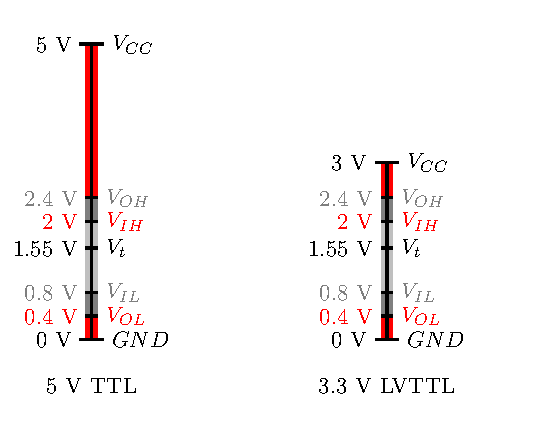
\includegraphics[width=.6\textwidth, page = 1]{ImagenesEjercicio4/Draw.pdf}
  \caption{Niveles Lógicos TTL y LVTTL}.
  \label{fig:ttlLvl}
\end{figure}
La segunda es la implementación de un Level Shifter mediante un transistor MOS y dos resistencias (\ref{fig:LVSH}), esta configuraicón permite la traducción de los niveles lógicos en ambos sentidos.
\begin{figure}[H]
  \centering
  \includegraphics[width=.6\textwidth, page = 2]{ImagenesEjercicio4/Draw.pdf}
  \caption{Level Shifter}.
  \label{fig:LVSH}
\end{figure}